% Created 2016-02-22 mån 14:31
\documentclass{beamer}
\usepackage[utf8]{inputenc}
\usepackage[T1]{fontenc}
\usepackage{fixltx2e}
\usepackage{graphicx}
\usepackage{longtable}
\usepackage{float}
\usepackage{wrapfig}
\usepackage{soul}
\usepackage{textcomp}
\usepackage{marvosym}
\usepackage{wasysym}
\usepackage{latexsym}
\usepackage{amssymb}
\usepackage{hyperref}
\tolerance=1000
\hypersetup{colorlinks= true, urlcolor= blue,linkcolor= none citecolor= red}
\providecommand{\alert}[1]{\textbf{#1}}

\title{Orthology analyses of 394 fungal proteomes}
\author{Elisabet Sjökvist}
\date{\today}
\hypersetup{
  pdfkeywords={},
  pdfsubject={},
  pdfcreator={Emacs Org-mode version 7.9.3f}}

\begin{document}

\maketitle

\begin{frame}
\frametitle{Outline}
\setcounter{tocdepth}{3}
\tableofcontents
\end{frame}


\begin{frame}
\frametitle{Project backgound}
\label{sec-1}

\begin{itemize}
\item How do pathogens evolve?
\begin{itemize}
\item how has the secretome evolved, and how does that differ between fungi with different nutritional strategies?
\item how has the effector repetoar evolved?
\item what is the composition of carbohydrate active enzymes and lignocellolytic enzymes?
\end{itemize}
\end{itemize}
  
\end{frame}
\begin{frame}
\frametitle{Genomes}
\label{sec-2}

\begin{itemize}
\item 564 genomes in Ensembl
\item 659 genomes in NCBI
\item 567 genomes in JGI, not all published
\item 394 publicly avaliable proteomes of ``different species''
\end{itemize}
\end{frame}
\begin{frame}
\frametitle{Orthology analyses}
\label{sec-3}
\begin{itemize}

\item All vs. all blast \~{} 4 weeks
\label{sec-3-1}%
\begin{itemize}
\item 395 fasta files
\item 395 blast databases
\item min. 30aa
\item max one stop codon at end of sequence
\end{itemize}

\item Orthofinder \~{} 9 days
\label{sec-3-2}%
\begin{itemize}
\item SequenceIDs.txt
\item SpeciesIDs.txt
\item 156025 blast result files
\end{itemize}
\end{itemize} % ends low level
\end{frame}
\begin{frame}
\frametitle{Distribution of cluster sizes}
\label{sec-4}

\begin{figure}[htb]
\centering
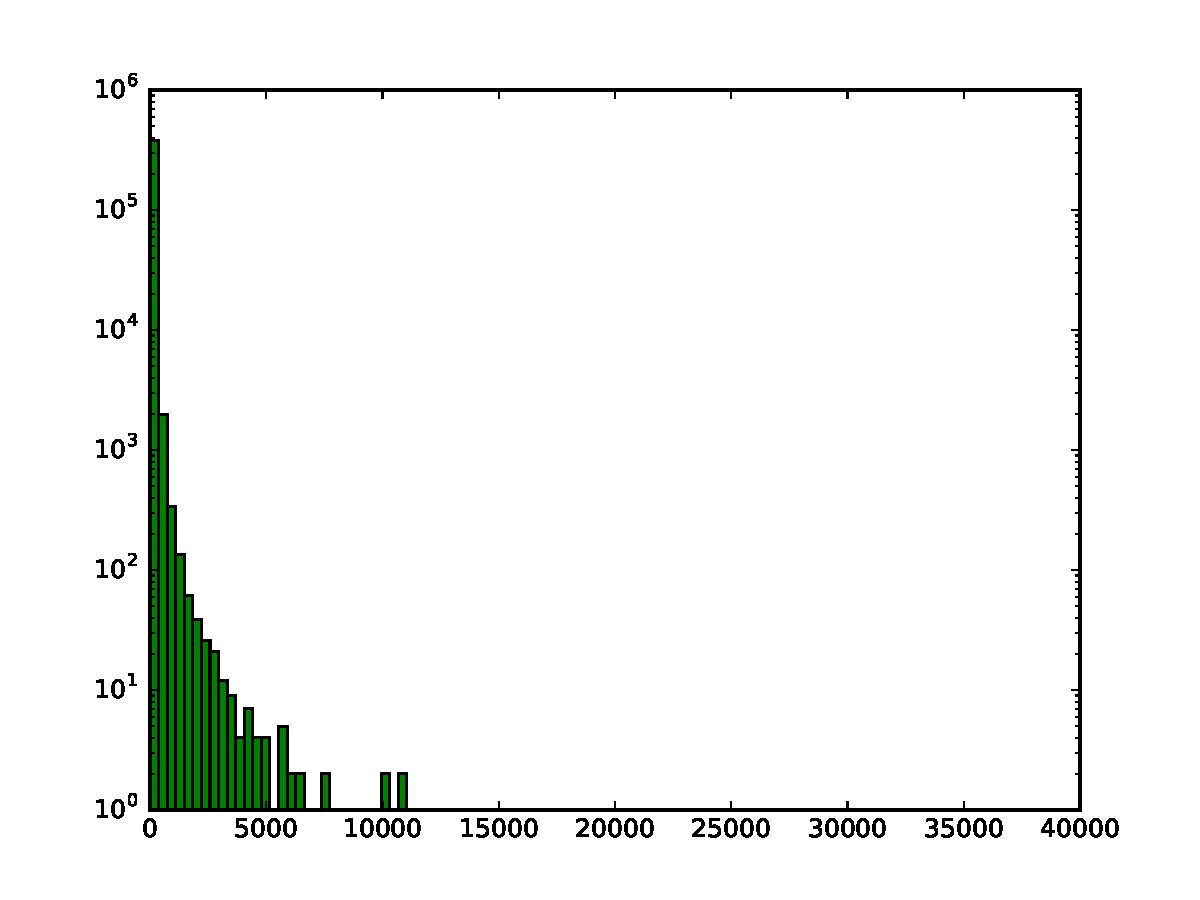
\includegraphics[width=.9\linewidth]{./proteins_per_cluster.pdf}
\caption{Distribution of cluster sizes, y-axis = nr of clusters, x-axis = proteins per cluster}
\end{figure}
\end{frame}
\begin{frame}
\frametitle{Database structure}
\label{sec-5}

\begin{figure}[htb]
\centering
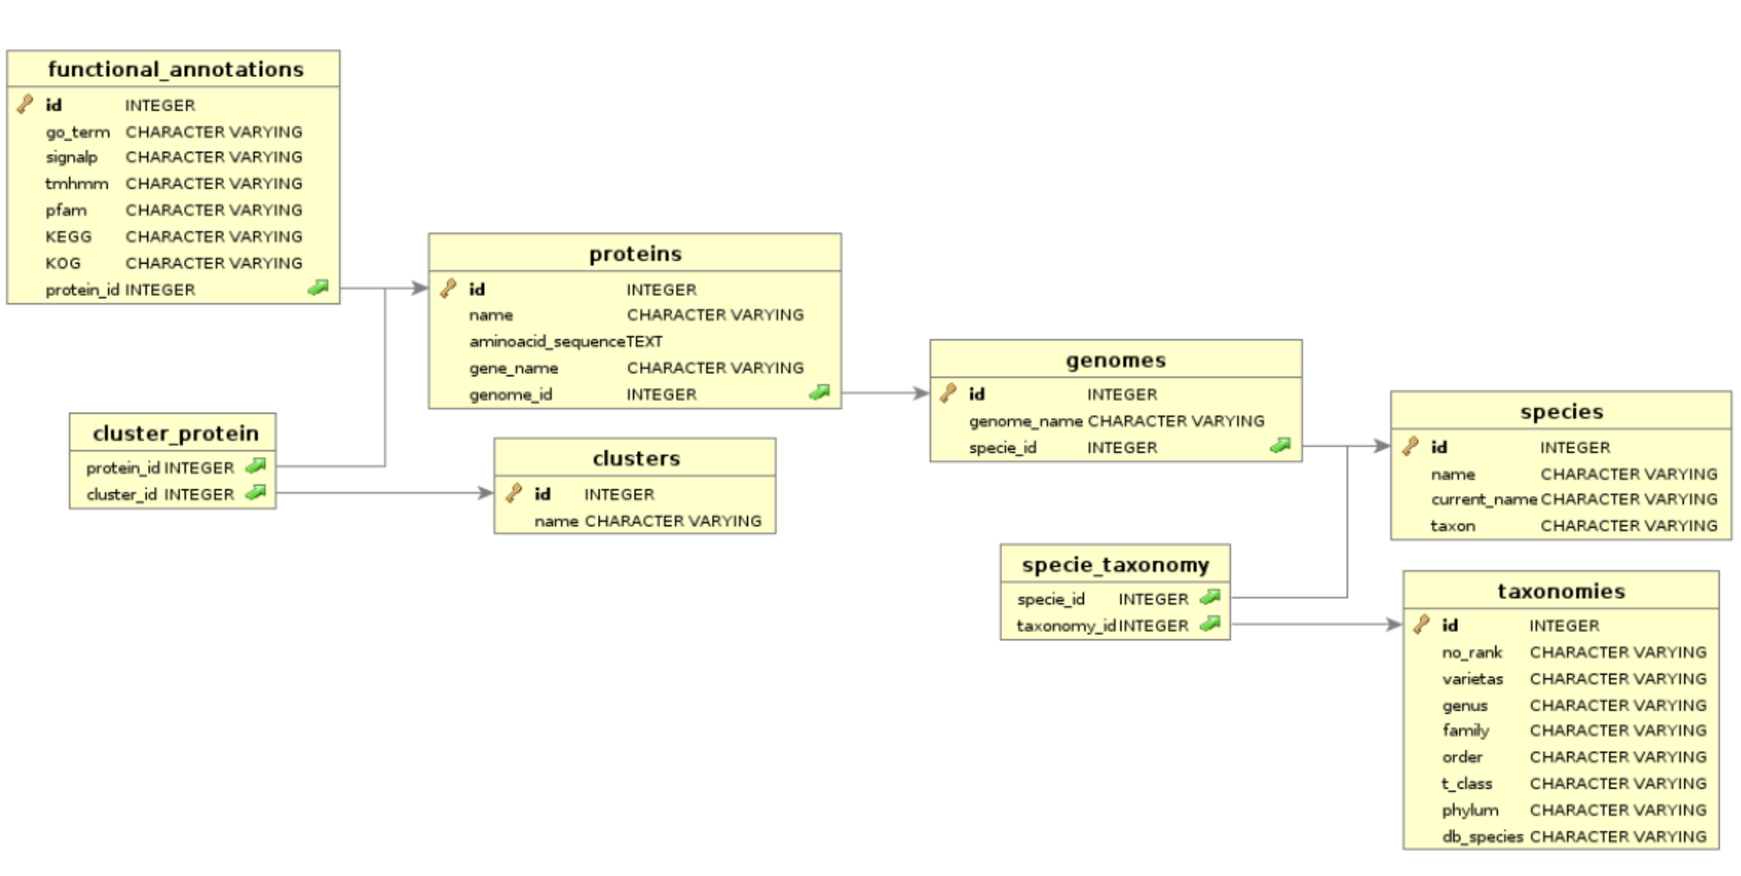
\includegraphics[width=.9\linewidth]{./presentation/database_structure_fun_395.pdf}
\caption{Organization}
\end{figure}
\end{frame}
\begin{frame}
\frametitle{Taxonomy                     ^}
\label{sec-6}

fun395=\# select count(taxonomies.id), taxonomies.phylum from taxonomies group by taxonomies.phylum;
 count |       phylum        
-------+---------------------
    11 | undef
     3 | Chytridiomycota
   234 | Ascomycota
     1 | Glomeromycota
    88 | Basidiomycota
    19 | Microsporidia
     1 | Blastocladiomycota
     1 | Cryptomycota
     1 | Entomophthoromycota
(9 rows)
\end{frame}
\begin{frame}
\frametitle{Nr. of protein families as a function of species sampled}
\label{sec-7}

\begin{itemize}
\item random sampling of 20-380 taxa with 20sp interval x 20
\item clusters where taxa have at least 1 protein present
\end{itemize}
\begin{figure}[htb]
\centering
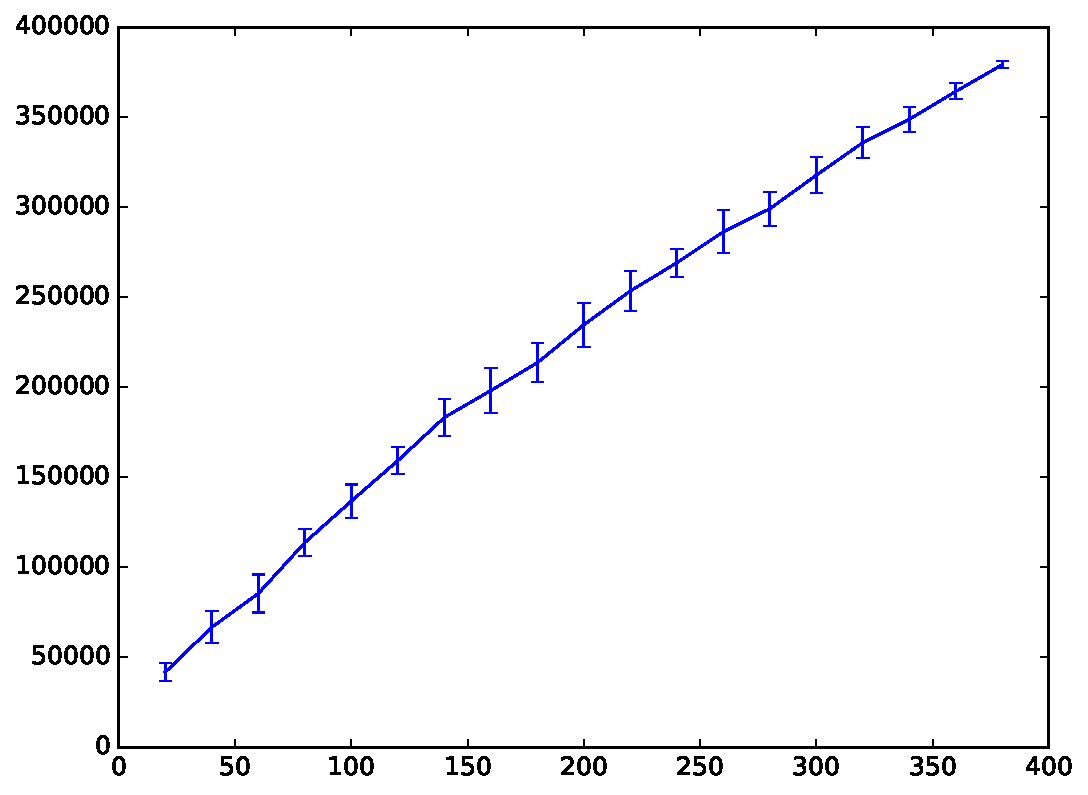
\includegraphics[width=.9\linewidth]{./gene_families_plotted.pdf}
\caption{y-axis nr of clusters/gene familes, x-axis species sampled}
\end{figure}
\end{frame}

\end{document}
